% Assembled for Overleaf: full paper with section rewrites spliced in and Gemini/Claude naming.
% Internal scratch comments (chunk banners, REVIEW block, PIN notes) stripped.

\documentclass[conference]{IEEEtran}
\IEEEoverridecommandlockouts
% The preceding line is only needed to identify funding in the first footnote. If that is unneeded, please comment it out.
\usepackage{cite}
\usepackage{amsmath,amssymb,amsfonts}
\usepackage{algorithmic}
\usepackage{graphicx}
\usepackage{textcomp}
\usepackage{xcolor}
\usepackage{comment}

\def\BibTeX{{\rm B\kern-.05em{\sc i\kern-.025em b}\kern-.08em
    T\kern-.1667em\lower.7ex\hbox{E}\kern-.125emX}}

\title{Strategic Reasoning Under Incomplete Information: Evaluating Frontier Language Models in Negotiation, Auctions, and Deception
% \footnotesize \textsuperscript{*}Note: Sub-titles are not captured in Xplore and should not be used
% \thanks{note}
}

\begin{comment}
\author{
\IEEEauthorblockN{Alexander Shang}
\IEEEauthorblockA{%\textit{dept. name of organization (of Aff.)} \\
\textit{Cosumnes Oaks High School}\\
Sacramento, CA \\
alexander.shang1101@gmail.com}
\and
\IEEEauthorblockN{Max Liu}
\IEEEauthorblockA{\textit{Clements High School} \\
%\textit{name of organization (of Aff.)}\\ 
Sugar Land, TX \\
maxliu2k@gmail.com}
\and
\IEEEauthorblockN{Eric Huang}
\IEEEauthorblockA{\textit{Westwood High School} \\
Austin, TX\\
erichuang0510@gmail.com}
\and
\IEEEauthorblockN{Ziliang Zong}
\IEEEauthorblockA{%\textit{Texas} \\
\textit{Texas State University}\\
San Marcos, TX \\
ziliang@txstate.edu}
}
\end{comment}

\begin{document}
\maketitle

\begin{abstract}

Strategic reasoning under incomplete information is a fundamental capability for autonomous agents operating in real-world environments. While frontier large language models (LLMs) have demonstrated strong performance on reasoning, planning, and coding tasks, their ability to negotiate, compete, and adapt strategically in multi-agent settings remains largely unknown. Existing evaluations primarily focus on static benchmarks and provide limited insight into how models behave when outcomes depend on hidden information, competing incentives, and repeated interactions. We introduce a unified evaluation framework for studying strategic reasoning in frontier language models across three representative environments: buyer-seller negotiation, sequential budget-constrained auctions, and repeated deception games. To enable scalable experimentation, we further propose \emph{behavioral mimics}, lightweight neural surrogates trained to reproduce the decision patterns of frontier LLMs at a fraction of the computational cost. We evaluate five state-of-the-art LLMs and analyze their behavior across strategic settings. Our results reveal that LLMs exhibit stable and human-interpretable behavioral signatures that can be distilled into compact surrogate models. However, these behaviors are often driven by simple heuristics rather than sophisticated strategic reasoning. In auctions, models converge toward reservation-price strategies that are exploitable by simple baselines. In deception settings, most models fail to calibrate dishonest behavior in response to declining credibility, leading to systematically suboptimal outcomes. We further show that distributionally faithful behavioral mimics do not necessarily preserve strategic rankings, highlighting an important limitation of surrogate-based evaluation. 

%Our findings provide new insights into the strategic capabilities and limitations of frontier language models and establish a scalable benchmark for evaluating agentic reasoning under incomplete information.

\end{abstract}

\begin{IEEEkeywords}
agentic AI, large language models, negotiation, strategy, multi-agent, incomplete information, reasoning
\end{IEEEkeywords}

\section{Introduction}

Large language models (LLMs) are increasingly being deployed as autonomous agents capable of planning, decision making, tool use, and interaction with other agents. As these systems move beyond isolated question-answering tasks and begin participating in real-world economic and social environments, their ability to reason strategically becomes increasingly important. Applications such as automated procurement, contract negotiation, resource allocation, market participation, and multi-agent coordination all require agents to make decisions under uncertainty while accounting for the incentives and behavior of others.

A defining characteristic of these environments is \emph{incomplete information}. Unlike classical planning tasks, agents rarely have direct access to their counterparts' preferences, constraints, intentions, or future actions. Therefore, success depends not only on reasoning about the environment itself, but also on reasoning about other agents. Strategic interaction under incomplete information has long been studied in economics, game theory, and multi-agent systems, where even simple settings can produce complex emergent behaviors. As LLM-based agents become increasingly capable, an important question arises: To what extent can frontier language models reason strategically when interacting with other agents under incomplete information?

Despite growing interest in agentic AI, existing evaluation methodologies provide only a partial answer. Most popular benchmarks focus on knowledge retrieval, mathematical reasoning, coding ability, or static planning tasks. Even recent agent-focused evaluations often emphasize task completion, tool use, or cooperative coordination rather than strategic competition. As a result, relatively little is known about how LLMs negotiate, allocate resources, adapt to opponents, manage credibility, or exploit strategic opportunities over extended interactions.

To address this gap, we introduce a unified evaluation framework for strategic reasoning under incomplete information. Rather than focusing on a single task, we evaluate models across three complementary environments that capture distinct aspects of strategic decision making:

\begin{itemize}
\item \textbf{Buyer-Seller Negotiation}, which evaluates bargaining behavior, agreement formation, and utility optimization under private valuations.
\item \textbf{Sequential Auctions}, which examine resource allocation, budget management, and competitive bidding dynamics.
\item \textbf{Repeated Deception Games}, which measure credibility management, strategic dishonesty, and long-term incentive reasoning.
\end{itemize}

Together, these environments provide a broader view of strategic intelligence than any individual task alone. Each environment introduces hidden information, competing incentives, and multi-step interactions that require agents to balance immediate rewards against future consequences.

A second challenge in evaluating strategic behavior is scalability. Large-scale experiments involving frontier LLMs are computationally expensive and often require thousands of sequential model calls. To address this challenge, we introduce \emph{behavioral mimics}: lightweight neural models trained to reproduce the decision patterns of individual LLMs. These surrogates enable large-scale experimentation at negligible cost while preserving key behavioral characteristics of the original models. This allows us to investigate not only how LLMs behave, but also whether their strategic behaviors can be distilled and reproduced by compact models.

Our empirical analysis reveals several consistent patterns. First, frontier LLMs exhibit stable and human-interpretable behavioral signatures that persist across repeated interactions. Second, many observed behaviors can be explained by relatively simple heuristics rather than sophisticated opponent modeling or adaptive strategic reasoning. Third, compact behavioral mimics successfully reproduce many observable behavioral distributions, suggesting that much of the strategic behavior exhibited by current LLMs is highly structured and predictable. Finally, we identify a critical limitation of surrogate-based evaluation: distributional fidelity does not necessarily imply strategic fidelity, and strategies that perform well against mimics may fail to transfer against the original language models.

These findings suggest that current frontier LLMs possess meaningful but limited strategic capabilities. While they can participate effectively in negotiation and competition, they often fail to adapt optimally to changing incentives, opponent behavior, or long-term consequences. Understanding these limitations is important both for deploying autonomous agents safely and for developing future systems capable of more robust strategic reasoning.

The contributions of this paper are as follows:

\begin{itemize}
\item We conduct a diverse study for evaluating strategic reasoning under incomplete information across negotiation, auction, and deception environments.
\item We propose behavioral mimics, lightweight surrogate models that reproduce LLM decision patterns and enable scalable strategic evaluation.
\item We provide a large-scale empirical analysis of strategic behavior in five frontier LLMs.
\item We demonstrate that distributional behavioral fidelity does not necessarily imply transferability of strategic performance, revealing an important limitation of surrogate-based evaluation.
\end{itemize}

\section{Related Works}

Strategic interaction under incomplete information has long been studied in economics, game theory, and multi-agent systems. Classical frameworks, such as Bayesian games model settings in which agents must make decisions without direct access to the preferences, constraints, or intentions of the other participants. These ideas later influenced research in autonomous agents and multi-agent reinforcement learning, where agents learn negotiation, cooperation, and competition strategies through repeated interaction. Prior work demonstrated that strategic behaviors can naturally emerge when agents are optimized for reward in environments with partially aligned incentives \cite{Leibo}. Similar findings appeared in communication-based multi-agent systems, where agents developed signaling strategies and adaptive communication protocols during interaction.

Recent advances in large language models have enabled the deployment of natural-language agents in strategic environments involving negotiation, persuasion, and long-term planning. Systems such as CICERO combine language generation with strategic reasoning to achieve human-level performance in the game of Diplomacy, demonstrating that language models can coordinate, negotiate, and reason over extended interactions \cite{Cicero}. More recent studies investigated LLM-based negotiation systems directly, including buyer-seller bargaining, adversarial negotiation, and multi-agent coordination tasks \cite{Abdelnabi}, \cite{PieArena}, \cite{AgenticPay}. These works suggested that frontier language models were increasingly capable of sophisticated strategic behavior, motivating systematic evaluation of how such models negotiate, allocate resources, and adapt to opponents under uncertainty.

At the same time, growing attention has been directed toward deceptive and strategically misleading behavior in language models. Deception has traditionally been defined as the intentional manipulation of another agent’s beliefs to influence behavior or outcomes \cite{Chisholm}, \cite{Faulkner}. Computational work extended these concepts into decision-theoretic environments by formalizing deception as a strategic policy that altered another agent’s belief state for competitive advantage \cite{Abdulhai}. Within modern LLM systems, researchers have observed that deceptive or selectively truthful behavior may emerge not from explicit programming, but from optimization incentives introduced during training. Reinforcement Learning from Human Feedback (RLHF), now widely used for aligning language models, optimizes outputs preferred by human evaluators \cite{Ouyang}. While effective for improving usability and helpfulness, such optimization may also reward persuasive or confidence-inducing responses even when those responses are incomplete or strategically framed. Subsequent work further explored how reward models and alignment procedures shaped model behavior \cite{Bai1}, \cite{Bai2}. Studies on deceptive alignment and conditional behavior additionally showed that models may adapt their responses depending on perceived oversight or evaluation conditions \cite{Greenblatt}, \cite{E. Hubinger}.

Evaluating these behaviors required benchmarks capable of measuring multi-turn interaction and strategic adaptation rather than isolated question-answer performance. Prior surveys on LLM evaluation argued that many existing benchmarks failed to capture long-term planning, adversarial reasoning, or dynamic interaction \cite{Chang}. In response, researchers have proposed interactive evaluation systems involving self-play, adversarial dialogue generation, and negotiation-based tasks \cite{Perez}. Several studies also used simulated multi-agent environments to generate large-scale dialogue datasets without extensive human annotation \cite{Abdullin}. Other work investigated the use of language models themselves as evaluators for conversational quality and strategic performance \cite{Zheng}. Together, these developments established the foundation for studying negotiation, deception, and strategic reasoning in realistic multi-agent environments.

Our work builds upon these prior directions by introducing a unified benchmark framework that evaluates frontier language models across multiple forms of strategic interaction, including negotiation simulations, sequential auctions, and deception-oriented persuasion tasks. Unlike prior work focused on a single environment or negotiation setting, our framework compares models across several other strategic domains while combining quantitative performance metrics with qualitative behavioral characterization. In addition, we introduce behavioral mimic models that enable scalable experimentation against deterministic strategic baselines, allowing large-scale analysis of emergent LLM negotiation and deception behavior.


\section{Methodology}


\subsection{Buyer-Seller Negotiation}

To study bargaining under asymmetric private constraints, we designed a bilateral negotiation in which two LLM agents must balance surplus extraction against the risk of leaving mutually beneficial gains unrealized. Each agent observes its own hard price bound and a short public interaction history, while the opponent's bound remains hidden. The setting exposes role-dependent offering, concession, acceptance, and walk-away behavior in a compact action space that can be logged at the turn level and distilled into behavioral mimics.

\subsubsection{Environment and Action Protocol}

We implement a finite bilateral alternating-offer game between a buyer $B$ and seller $S$. The buyer privately observes a hard budget $v_B$ and a target-price prompt anchor; the seller privately observes a hard reservation floor $v_S$ and an opening-ask anchor. Let $\mathsf{U}_{\mathbb{Z}}[a,b]$ denote the discrete uniform distribution on the integers from $a$ to $b$. The engine first samples $v_S\sim\mathsf{U}_{\mathbb{Z}}[85,175]$, then samples one of three valuation regimes:
\begin{equation}
v_B\sim
\begin{cases}
\mathsf{U}_{\mathbb{Z}}[v_S,b_f], & \text{feasible},\\
\mathsf{U}_{\mathbb{Z}}[v_S,b_t], & \text{tight},\\
\mathsf{U}_{\mathbb{Z}}[\ell_i,u_i], & \text{infeasible},
\end{cases}
\end{equation}
where $b_f=\min(220,v_S+70)$, $b_t=\min(220,v_S+15)$, $\ell_i=\max(40,v_S-35)$, and $u_i=\max(40,v_S-5)$. The seller's initial ask anchor is $v_S+\mathsf{U}_{\mathbb{Z}}[8,55]$; the buyer target is its budget minus a random amount in $[0,28]$, subject to the engine's lower bound. The experiments reported in Section~IV-A use only the \emph{feasible} regime. Tight and infeasible regimes are implemented for the expanded rejection study but are not included in the reported estimates.

The seller sends the first message, which the engine constrains to be an offer, and the parties then alternate for at most $H=8$ total messages. On later turns the acting model selects
\begin{equation}
a_t\in\{\texttt{continue}(p_t),\texttt{accept},\texttt{reject}\}.
\end{equation}
Each live-model prompt contains the acting role's private bound and anchor, the current standing offer, an explicit deadline counter, and up to the six most recent public offers/messages; it never contains the opponent's private bound. Calls use temperature $0.2$ and a structured action schema. The engine parses the reply and applies a legality layer: buyer proposals are clipped to $[1,v_B]$, seller proposals to $[v_S,9999]$, and accept is legal only when the standing offer respects the acting agent's bound. Accept closes at the standing price, reject ends immediately with no deal, and exhausting the message limit produces a timeout. The recorded behavior is therefore the canonical action after parsing and legality enforcement---the LLM-plus-wrapper policy---rather than unconstrained text.

For agreement at price $p$, utilities are $U_B=v_B-p$ and $U_S=p-v_S$; both are zero without agreement. Let $G=v_B-v_S$ denote available bargaining surplus. For $G>0$ we report
\begin{equation}
z=\frac{p-v_S}{G},\qquad
u_B=\frac{U_B}{G},\qquad
u_S=\frac{U_S}{G},
\end{equation}
where $z=0$ gives the buyer all available surplus and $z=1$ gives it to the seller. Zero- or negative-surplus episodes have no normalized price and are evaluated by their terminal outcome.

\subsubsection{Live-Model Data and State Encoding}

The source population comprises GPT-5.4, Grok 4.3, Llama 4 Maverick, Claude Opus 4.6, and Gemini 3.1 Pro. We run all $5\times5=25$ directed buyer--seller pairings once under each of ten matched environment seeds. Holding the seed fixed presents identical private values to every pairing, yielding 250 live-model episodes and 1{,}060 canonical turn decisions: 811 continue, 218 accept, and 31 explicit reject. Each completed log records model and role, seed, both private bounds for offline outcome analysis, the public offer sequence, canonical action, termination reason, and final price.

The mimic input is a leakage-safe 32-dimensional pre-action vector. It encodes role; turn and remaining-message fractions; the acting agent's private bound and target; presence, level, and change of the standing offer; counts and summary statistics of public prices; separate own and opponent offer counts, best offers, and total/last concessions; the latest buyer--seller gap; and first/deadline indicators. Monetary features are expressed either relative to the acting agent's private bound or on a fixed \$1{,}000 scale. Opponent private values, the current action, terminal outcome, final price, and message text are excluded. Buyer and seller examples share a model-specific network because role is included in the state vector.

\subsubsection{Mimic Training and Deployment}

For each source LLM we train a single role-conditioned network with a shared trunk and two output heads. The trunk is two fully-connected layers of width $64$ with Tanh activations ($32\!\to\!64\!\to\!64$); from its representation an action head ($64\!\to\!3$) emits logits over continue, accept, and reject, and a price head ($64\!\to\!1$) emits the proposed price as a fraction of the acting agent's private bound. The action head is trained with weighted cross-entropy: for class $c$ with $n_c>0$ training examples, the fold-specific weight is
\begin{equation}
w_c=\min\!\left(3,\sqrt{n_{\max}/n_c}\right),
\end{equation}
which raises the influence of terminal actions without fully inverse-weighting the 31 sparse rejects. The price head is trained only on continue actions, using Huber loss ($\delta=0.1$). Inputs are standardized using training-fold statistics. Training uses AdamW (learning rate $10^{-3}$, weight decay $10^{-4}$), batch size 32, at most 300 epochs, and early stopping with patience 40.

All splits are grouped by environment seed. For each cross-fitted checkpoint, one seed is held out for testing and a second seed from the remaining pool is used for early stopping; no turn from the test valuation scenario enters that checkpoint's training or validation data. Seeds 0--4 form the rollout-development subset used to select deployment stochasticity, while fidelity is reported on seeds 5--9. The selection objective is the sum of terminal-outcome total-variation distance (TVD), absolute agreement-rate gap, and conditional-price Wasserstein distance on development rollouts. It selects action temperature $0$ (argmax after masking illegal actions) and price temperature $0.5$. For a continue action, deployment adds zero-mean Gaussian noise at one half of the model-specific training-residual standard deviation, then clips the resulting offer to the legal interval.

\subsubsection{Fidelity and Baseline Protocol}

Decision-level fidelity scores the five evaluation seeds with the corresponding seed-held-out checkpoints and reports accuracy, macro-F1, per-class recall, action-distribution TVD, and conditional offer-price MAE. Outcome-level fidelity compares the 125 real episodes on seeds 5--9 with three mimic replicates of every matched seed/pairing, for 375 mimic episodes. We report agreement, explicit rejection, timeout, normalized utilities, conditional $z$, message count, terminal-outcome TVD, and conditional-price Wasserstein distance. The environment seed is the independent unit: bootstrap intervals use 4{,}000 resamples of seeds and retain all pairings and mimic replicates within a sampled seed.

For baseline screening, each mimic plays both buyer and seller against a deterministic mathematical policy over the same five evaluation seeds and three mimic replicates, giving 15 episodes per model/role cell. The mathematical policy estimates an opponent bound from public offers, scores candidate prices with a smooth acceptance model and a deadline-dependent no-deal cost, and accepts when the standing offer is competitive with its best counteroffer; it does not explicitly reject. We additionally report mathematical self-play. These comparisons are mimic-mediated: because the baseline has not yet been run against the real LLMs, Section~IV-A does not claim that its ranking transfers.

\subsection{Multi-Agent Auction}
To investigate LLMs' behavior in a constrained strategic setting, we designed a sequential open-ascending auction over twelve identical paintings. Five bidders compete in turn order, each starting with a budget of \$10,000. On each turn a bidder either raises the current bid (subject to a tiered minimum-raise schedule) or passes, with passes being permanent for the current painting. A painting resolves when only one active bidder remains; that bidder pays their final bid and wins the painting. The objective is to win as many paintings as possible; money is worthless in the reward function. Because the paintings are undifferentiated, the strategic problem is purely one of budget allocation and timing: when to commit, when to fold, and how to respond to opponents' commitments.
%Formally this is a finite sequential open-ascending (English) auction with budget-constrained bidders and irrevocable exit (a bidder that passes cannot re-enter for the current lot). When bids advance by the minimum increment (as our deterministic baselines do by construction, and the LLMs do on the large majority of turns), the mechanism coincides with a Japanese button auction, in which a bidder's play reduces to a \emph{reservation-price} (drop-out) strategy: a state-dependent price at which it leaves the contest for the current lot~\cite{MilgromWeber}. This setting lets us compare LLM bidders against principled deterministic policies that operate over the same observable state, defined in Section~\ref{sec:auction-baselines}.

\subsubsection{Behavioral Mimics}
\label{sec:mimics}
Running the baseline comparison against real LLMs is prohibitively slow and costly: a single auction makes hundreds of sequential model calls (roughly 70 per bidder), so the full sweep of hundreds of auctions across policies and seeds would run into hundreds of dollars and tens of hours, repeated on every change. We therefore train a \emph{behavioral mimic} of each LLM from a sample of real auctions and use the mimics as essentially free drop-in replacements at scale.
%The tradeoff is explicit: we are no longer testing the LLMs directly, but networks trained to reproduce their behavior over the auction state space; Section~\ref{sec:fidelity-results} quantifies how faithful that substitution is.

\subsubsection{Mimic Architecture and Training}
For each of the five LLMs, we train a pair of networks on a common encoding of the auction state. At the decision point of bidder $i$ on turn $t$, the public information is encoded as a normalized feature vector $\mathbf{x}^i_t \in \mathbb{R}^{32}$ formed by concatenating five blocks,
\begin{equation}
\mathbf{x}^i_t = \big[\, \mathbf{x}_{\mathrm{prog}} \,\Vert\, \mathbf{x}_{\mathrm{round}} \,\Vert\, \mathbf{x}_{\mathrm{self}} \,\Vert\, \mathbf{x}_{\mathrm{prev}} \,\Vert\, \mathbf{x}_{\mathrm{opp}} \,\big],
\end{equation}
where $\Vert$ denotes concatenation and budgets are normalized by $B_0 = \$10{,}000$. With $n_t$ paintings remaining, minimum legal bid $\underline{b}_t$, opponent budgets $\{B^j_t\}$, and paintings won $\{w^j_t\}$, the five blocks (with dimensions) are progress ($\mathbf{x}_{\mathrm{prog}}\in\mathbb{R}^{3}$: paintings elapsed and a last-lot flag), round state ($\mathbf{x}_{\mathrm{round}}\in\mathbb{R}^{4}$: current and minimum legal bids, active bidders, and turn count), the bidder's own position ($\mathbf{x}_{\mathrm{self}}\in\mathbb{R}^{7}$: its budget in absolute, relative, and fair-share terms, paintings won, deficit to the leader, and standing bid), its previous action ($\mathbf{x}_{\mathrm{prev}}\in\mathbb{R}^{3}$), and opponent summaries ($\mathbf{x}_{\mathrm{opp}}\in\mathbb{R}^{15}$: order statistics of opponent budgets and win counts), concatenating to $32$ dimensions.
The two heads map this vector to a bid. A classifier $f_\theta : \mathbb{R}^{32} \to [0,1]$ outputs the raise probability $p^i_t = f_\theta(\mathbf{x}^i_t)$, and a regressor $g_\psi : \mathbb{R}^{32} \to \mathbb{R}_{\ge 0}$ outputs the overbid $\delta^i_t = g_\psi(\mathbf{x}^i_t)$ above $\underline{b}_t$, measured in units of the legal raise increment $\Delta_t$. The emitted action, over the legal set $\mathcal{A}_t = \{\texttt{pass}\} \cup \{\texttt{raise}(v) : v \ge \underline{b}_t\}$, is
\begin{equation}
a^i_t =
\begin{cases}
\texttt{pass}, & u^i_t = 0,\\[2pt]
\texttt{raise}\big(\underline{b}_t + \lfloor \delta^i_t \rceil\, \Delta_t\big), & u^i_t = 1,
\end{cases}
\end{equation}
where $\lfloor\cdot\rceil$ rounds to the nearest non-negative integer number of steps and $u^i_t \in \{0,1\}$ is the raise decision drawn from $p^i_t$ (sampled with temperature at deployment, as described below).

The classifier is an MLP with two hidden layers of width 32 ($32\!\to\!32\!\to\!32\!\to\!1$), sigmoid activations, and dropout $0.2$, trained with binary cross-entropy. The regressor shares this shape with ReLU activations and a softplus output, trained with Huber loss on the subset of rows where the LLM raised. We fit the mimics on 3{,}334 decisions from the ten real auctions, using leave-one-episode-out cross-validation as an honest accuracy check and excluding earlier mimic-vs-mimic runs to avoid self-feedback. At deployment the mimics act \emph{stochastically}, sampling the raise/pass decision and perturbing the overbid under a temperature parameter, so they reproduce the source policy's variance rather than collapsing to its modal action.

\subsubsection{Fidelity Validation Procedure}
We validate the substitution at two levels. At the \emph{outcome} level we run real-LLM and mimic auctions under identical conditions and compare the resulting distributions of paintings won, treating the auction as the independent replicate and reporting the effect size (Cram\'er's $V$) together with auction-level bootstrap confidence intervals on the per-model win-share differences, plus a chi-squared test of independence as a secondary check. At the \emph{decision} level we report the leave-one-episode-out cross-validation accuracy of the raise/pass classifier and the overbid regressor's mean absolute error. Results are reported in Section~\ref{sec:fidelity-results}.

\subsubsection{Deterministic Baseline Policies}
\label{sec:auction-baselines}
We compare against four hand-coded heuristics and one learned policy, all acting on the same observation $\mathbf{x}^i_t$ and emitting an action $a^i_t \in \mathcal{A}_t$. The four heuristics never overbid: when they act they raise to exactly the minimum legal bid $\underline{b}_t$, so their only decision is when to pass. Each is thus a reservation-price (drop-out) strategy, specified by a state-dependent willingness-to-pay cap $c^i_t$, and follows
\begin{equation}
a^i_t =
\begin{cases}
\texttt{raise}(\underline{b}_t), & \underline{b}_t \le \min(c^i_t,\, B^i_t),\\[2pt]
\texttt{pass}, & \text{otherwise.}
\end{cases}
\end{equation}
The caps form a ladder of increasing information use. With deficit-to-leader $d^i_t$, catch-up factor $\kappa^i_t = 1 + 0.18\,d^i_t$, and endgame factor $\eta_t = 1.75$ for $n_t \le 3$, $1.15$ for $3 < n_t \le 6$, and $1$ otherwise:
\begin{itemize}
\item \textbf{Trivial:} $c^i_t = \infty$. Raises whenever solvent; no state, no opponent reasoning. The ``do anything'' floor.
\item \textbf{Fair-Share:} $c^i_t = 1.05\,B^i_t / n_t$. Spreads its own budget evenly across remaining paintings; no opponent information.
\item \textbf{Reactive:} $c^i_t = (B^i_t / n_t)\,\kappa^i_t\,\eta_t$. Scales the fair share by the public scoreboard (win counts), but not opponent budgets.
\item \textbf{Market-Clearing:} $c^i_t = m_t\,\kappa^i_t\,\eta_t$, where the competitive-equilibrium price $m_t = \tfrac{1}{n_t}\sum_{j} B^j_t\,\mathbb{1}[B^j_t \ge \underline{b}_t]$ sums over all solvent bidders $j$ (including $i$). Adds opponent-budget visibility; because that base includes $i$ itself, it is by construction never less aggressive than Reactive.
\end{itemize}

The fifth policy, \textbf{RL}, replaces the hand-coded rule with a learned stochastic policy $a^i_t \sim \pi_\phi(\cdot \mid \mathbf{x}^i_t)$ trained with PPO (clipped surrogate objective, GAE advantage estimation) for 4{,}000 episodes against the mimic ensemble. Each episode randomizes the learner's seat and samples four of the five mimics as opponents; the reward is the number of paintings won, so the policy approximates a best response to the mimic opponent population.

\subsubsection{Experimental Design}
Each baseline is evaluated in 50 auctions in which it occupies one seat and four mimics fill the rest, with the displaced mimic rotated so that each of the five is replaced an equal number of times; this yields 600 contested paintings per baseline. Seeds and seat permutations are varied across auctions to control for turn-order effects. With five equal bidders, a strategically neutral policy wins the fair share of $20\%$. To test whether these mimic-mediated results transfer, we additionally run each baseline against the five real LLMs (5 auctions, 60 paintings, per baseline). Throughout, a policy's win rate is reported as the mean of its per-auction win fractions with an auction-level $95\%$ confidence interval, since the auction (not the individual painting) is the independent replicate; the $n=5$ transfer intervals are only indicative.

\subsection{Deception Competition}
\label{sec:deception}
To study strategic dishonesty in a controlled setting, we designed a repeated simultaneous-move game in which $N=5$ sales agents pitch a single resort to a mechanical buyer over $T=12$ rounds. Each round the resort is described by $K=5$ quality attributes whose true values form a vector $t^{(r)}\in[0,1]^{K}$, quantized to two decimal places and re-sampled each round, and every agent observes the full truth before acting. Each agent then simultaneously emits a claim vector $c_i^{(r)}\in[0,1]^{K}$. Because every agent sees the truth, a claim above it is a deliberate over-statement rather than a guess, so the game is purely one of how far each agent will distort what it knows, given that distortion erodes its standing with the buyer. The buyer is non-strategic (a fixed mechanism), and all five attributes are weighted equally.

\subsubsection{Scoring and booking}
The buyer scores each agent by its credibility-weighted appeal, where a per-attribute credibility $\mathrm{tr}_{i,a}^{(r)}\in[0,1]$ (initialized to $1$) multiplies each claim:
\begin{equation}
s_i^{(r)} = \frac{1}{K}\sum_{a=1}^{K} c_{i,a}^{(r)}\,\mathrm{tr}_{i,a}^{(r)}.
\label{eq:dec5-score}
\end{equation}
Per-attribute credibility acts as an attribute-level discount: a claim on a discredited attribute contributes little to the score even when it is high. Each round the buyer books the highest-scoring agent, $\mathcal{W}^{(r)}=\operatorname*{arg\,max}_i s_i^{(r)}$ (set-valued under ties, with no minimum threshold); winners split a unit reward equally and all others receive $0$, so an agent's episode return is its number of (tie-shared) bookings, bounded by $T$. The score magnitude never enters the reward directly; credibility matters only through who wins.

\subsubsection{Credibility dynamics: a track record}
The single cost of lying is a persistent loss of credibility, and it is incurred only on the rounds the buyer actually books the agent, since the buyer experiences a resort only when it books it. Writing the per-attribute over-promise as $d_{i,a}^{(r)} = \max\!\bigl(0,\, c_{i,a}^{(r)} - t_a^{(r)}\bigr)$, an agent's per-attribute credibility is one minus its average over-promise across the rounds it has won:
\begin{equation}
\mathrm{tr}_{i,a} = 1 - \frac{\sum_{r\,:\,i\in\mathcal{W}^{(r)}} d_{i,a}^{(r)}}{\max\!\bigl(1,\ n_i^{\mathrm{win}}\bigr)},
\label{eq:dec5-trust}
\end{equation}
where $n_i^{\mathrm{win}}$ is the agent's booking count so far. An agent that has never been booked retains full credibility (no track record). Winning a round with a large over-promise on attribute $a$ craters that attribute's credibility; winning with honest claims on $a$ heals it, since the running average falls. Because the denominator is the booking count and the numerator is per-attribute, the five-dimensional structure carries real strategic weight: a single-attribute lie damages only that dimension, so \emph{which} attribute to inflate, and how cheaply, is the core decision.

\subsubsection{Behavioral metrics}
We summarize an agent's revealed strategy by its lie rate (the fraction of claimed attributes that exceed the truth), its win rate (the fraction of rounds booked), its per-attribute over-promise $d_{i,a}^{(r)}$, and its final credibility $\mathrm{tr}_{i,a}^{(T)}$.

\subsubsection{Math-tier reference policies}
\label{sec:dec5-tiers}
Paralleling the auction baselines, we define a ladder of policies of increasing information use, all acting on the truth plus the listed state and emitting a quantized claim vector:
\begin{itemize}
\item \textbf{Trivial-Max:} claim $1.0$ on every attribute every round. No information; the state-free ceiling baseline.
\item \textbf{Truth-Anchored:} information $\{$truth$\}$. Claims maximally only where the truth is already high, so the over-promise (and thus the credibility damage) is small, and stays near the truth on the rest. The first ``thinking'' tier.
\item \textbf{Self-Aware:} adds own per-attribute credibility, own bookings, and round progress. Backs off inflation on attributes whose credibility is burned and restores them by claiming honestly there.
\item \textbf{Pack-Aware:} adds the opponents' credibility and bookings, concentrating inflation where it can outscore the current field.
\item \textbf{RL:} a stochastic policy warm-started by $30$ episodes of behavior cloning on Pack-Aware and then trained with PPO (clipped surrogate objective, GAE advantage estimation) for $8{,}000$ episodes against the mimic ensemble; the reward is the number of bookings, so the policy approximates a best response to the mimic opponent population.
\end{itemize}

\subsubsection{Behavioral mimics}
\label{sec:dec5-mimics}
As in the auction study, we distill each LLM into a cheap surrogate and use it as a drop-in replacement at scale. We reuse the two-head design of Section~\ref{sec:mimics}: a shared trunk feeding a lie head (a per-attribute probability of over-claiming, trained with binary cross-entropy) and a claim head (the regressed claim value, trained with mean-squared error on the attributes that were lied on). The only deception-specific change is the input, a leakage-safe $32$-dimensional encoding of the observed truth, the agent's own and opponents' per-attribute credibility, the round fraction, and a compact behavioral-history block, the last of which lets the surrogate reproduce timing-dependent play. At deployment the mimic samples the per-attribute lie decision (with temperature $\Theta$), snaps the attributes it does not lie about to the truth, and perturbs each remaining regressed claim by Gaussian noise at the claim head's per-attribute training-residual scale, so the surrogate reproduces the spread of each model's claims rather than collapsing to the conditional mean.

\subsubsection{Fidelity validation and the transfer test}
\label{sec:dec5-fidelity-method}
We validate the substitution at the level the mimics are actually used for, namely as the opponent field in the strategy comparison, and therefore at the \emph{outcome} level: we compare the per-model distribution of bookings between real-LLM and mimic-field games, treating the episode as the independent replicate. As a secondary and looser check we report the marginal claim-distribution total-variation distance (TVD). Finally, because distributional fidelity need not imply that strategy \emph{rankings} measured against the mimics hold against the real models, we run an explicit transfer test: each reference policy is played against a fixed field of mimics and, separately, against the real LLMs, and the two orderings are compared. Throughout, the episode is the independent replicate and win rates are reported as the mean of per-episode booking fractions with $95\%$ confidence intervals.

\section{Experimental Results}


\subsection{Buyer-Seller Negotiation}

\subsubsection{Model Behavior Characterization}

Table~\ref{tab:neg_behavior} characterizes each source model in both roles on the five held-out seeds (25 episodes per model/role). The buyer and seller columns are not symmetric duplicates: they measure the source model against all five opponents while occupying the indicated role. Grok and Claude are the strongest buyers, achieving nearly identical agreement ($92\%$) and normalized buyer utility ($0.661$ and $0.658$); their accepted prices allocate only $z=0.282$ and $0.285$ of the available surplus to the seller. In the seller role, GPT, Grok, and Claude form a middle cluster near $u_S=0.43$--$0.44$. Gemini closes most often as seller ($96\%$) but captures only $u_S=0.194$ and $z=0.202$, a high-closure, buyer-favorable signature. Llama is the clearest outlier: as seller it agrees in only $72\%$ of episodes and explicitly rejects $28\%$, compared with $4$--$12\%$ rejection for the other seller profiles.

\begin{table}[htbp]
\caption{Real-LLM negotiation behavior on held-out seeds. $AR_B$ and $u_B$ evaluate a model as buyer; $AR_S$ and $u_S$ evaluate it as seller. Utilities are normalized by available surplus and include zero for no deal ($n=25$ episodes per model/role; five independent seeds).}
\label{tab:neg_behavior}
\centering
\begin{tabular}{lcccc}
\hline
Model & $AR_B$ (\%) & $u_B$ & $AR_S$ (\%) & $u_S$ \\
\hline
GPT-5.4 & 92 & 0.498 & 92 & 0.434 \\
Grok    & 92 & 0.661 & 92 & 0.434 \\
Llama   & 80 & 0.350 & 72 & 0.296 \\
Claude  & 92 & 0.658 & 88 & 0.438 \\
Gemini  & 84 & 0.437 & 96 & 0.194 \\
\hline
\end{tabular}
\end{table}

\subsubsection{Mimic Fidelity}
\label{sec:neg-fidelity}

At the decision level, cross-fitted mimics recover $85.0\%$ of the 566 held-out actions (macro-F1 $0.518$). Continue and accept recall are $0.946$ and $0.582$, and the conditional offer-price MAE is \$13.3 (0.083 in own-bound ratio units). Explicit rejection is the unresolved class: recall is zero on 15 held-out reject actions. This is not hidden by the high aggregate accuracy, which is dominated by continue decisions.

At the rollout level the principal aggregates align much more closely than in the unweighted mimic. Agreement is $88.0\%$ for 125 real episodes and $89.3\%$ for 375 matched mimic episodes, a $+1.3$ percentage-point difference whose seed-clustered $95\%$ interval includes zero (Table~\ref{tab:neg_fidelity}). Conditional deal splits are also close ($z=0.408$ vs. $0.388$; Wasserstein distance $0.034$). Terminal-outcome TVD is $0.069$ with a wide five-seed interval $[0.045,0.200]$. The remaining mismatch is interpretable: mimics explicitly reject in $5.1\%$ of episodes versus $12.0\%$ for real models and take about $0.62$ more messages. Thus the surrogate is faithful for aggregate closure and price screening, but not yet for the mechanism of walking away.

\begin{table}[htbp]
\caption{Negotiation rollout fidelity. Differences and intervals are mimic minus real; intervals resample the five seeds while retaining all pairings and mimic replicates. Deal price $z$ is conditional on agreement.}
\label{tab:neg_fidelity}
\centering
\begin{tabular}{lccc}
\hline
Metric & Real & Mimic & Comparison \\
\hline
Agreement rate & 0.880 & 0.893 & $+0.013$ [$-0.075,0.155$] \\
Explicit rejection & 0.120 & 0.051 & $-0.069$ [$-0.200,0.021$] \\
Deal price $z$ & 0.408 & 0.388 & $W_1=0.034$ \\
Messages & 4.528 & 5.147 & $+0.619$ [$0.051,1.137$] \\
\hline
\end{tabular}
\end{table}

\subsubsection{Baseline Comparison}

Table~\ref{tab:neg_baseline} screens each mimic against the deterministic mathematical policy in both roles (15 episodes per cell: five seeds and three mimic replicates). Buyer performance separates sharply: Claude and Grok retain $u_B=0.742$ and $0.737$, with seed-clustered intervals $[0.595,0.870]$ and $[0.610,0.887]$, while Gemini reaches only $0.288$. Grok is also the strongest seller ($u_S=0.609$); Llama and Gemini concede most of the surplus as sellers ($0.253$ and $0.170$). Mathematical self-play always agrees, with $z=0.412$, allocating normalized utilities $u_B=0.588$ and $u_S=0.412$. These are mimic-mediated screening results. Unlike the auction and deception ladders, they have not yet been repeated against the real LLMs, so we do not claim that the ranking transfers.

\begin{table}[htbp]
\caption{Mimic performance against the mathematical policy. $u_B$ is the focal mimic as buyer; $u_S$ is the focal mimic as seller. Each cell has 15 episodes but only five independent seeds.}
\label{tab:neg_baseline}
\centering
\begin{tabular}{lcccc}
\hline
Mimic & $AR_B$ (\%) & $u_B$ & $AR_S$ (\%) & $u_S$ \\
\hline
GPT-5.4 & 100.0 & 0.469 & 93.3 & 0.422 \\
Grok    & 100.0 & 0.737 & 100.0 & 0.609 \\
Llama   & 100.0 & 0.432 & 100.0 & 0.253 \\
Claude  & 100.0 & 0.742 & 93.3 & 0.435 \\
Gemini  & 86.7 & 0.288 & 86.7 & 0.170 \\
\hline
\end{tabular}
\end{table}

\subsubsection{Synthesis}

The negotiation results reveal stable role-dependent signatures rather than one universally strong model: Grok and Claude extract buyer surplus, Gemini trades seller surplus for closure, and Llama walks away most readily. Capped class weighting corrects the v1 mimics' aggregate closure deficit without materially disturbing the deal-price distribution, bringing real and mimic agreement within $1.3$ percentage points. The unresolved boundary is explicit rejection and trajectory length, both rare-event, compounding-error problems. Consequently, the present mimics support price characterization and low-cost baseline screening, but not training a deployable negotiation policy or asserting baseline transfer. The next experiment therefore adds tight and infeasible bargaining regimes, more independent seeds, and real-LLM baseline transfer runs; these conditions supply genuine rejection examples instead of synthetically oversampling the 31 rejects in the current training set.

\subsection{Multi-Agent Auction}

\subsubsection{Model Behavior Characterization}
We characterize LLM bidding from ten real auctions. For this scenario we used five models with no special instructions: GPT, Claude, Gemini, Grok, and Llama. A striking feature is that all five reason from the same scaffold (an explicit per-painting ``fair-share'' computation stated in their own deliberations) yet derive very different behavior from it. Four of the five anchor to their own budget divided by the paintings ($10{,}000/12 \approx \$833$); Gemini instead anchors to the total money in the room divided by the paintings ($50{,}000/12 \approx \$4{,}166$), a five-fold higher valuation that leads it to read nearly every lot as underpriced. The models are far less differentiated in \emph{engagement} than in \emph{budget aggression}: all five participate on $95$--$97\%$ of paintings and bid the minimum increment on most turns (median raise \$50). Table~\ref{tab:auction_behavior} summarizes the per-model outcome and spending, ordered by paintings won.

\begin{table}[htbp]
\caption{Per-model auction behavior over ten real auctions: paintings-won share, the per-painting valuation anchor each model reasons from in its own deliberations, and mean budget spent per auction. Every model but Gemini anchors to its own budget divided by the lots ($\sim$\$833); Gemini anchors to the total money in the room ($\sim$\$4{,}166).}
\label{tab:auction_behavior}
\centering
\begin{tabular}{lccc}
\hline
Model & Win share (\%) & Anchor (\$) & Mean spend (\$) \\
\hline
Llama & 26.7 & 833   & 5{,}226 \\
Gemini & 21.7 & 4{,}166 & 7{,}495 \\
Claude & 18.3 & 833   & 6{,}955 \\
GPT   & 17.5 & 833   & 3{,}980 \\
Grok  & 15.8 & 833   & 5{,}890 \\
\hline
\end{tabular}
\end{table}

The spend column carries the efficiency story the win shares alone do not. Llama converts the highest win share from the second-lowest spend, the most budget-efficient profile, pairing assertive early bidding with a few large closing jumps. Gemini spends the most and throws the largest non-incremental jumps (single raises from \$100 into the thousands), buying wins at the cost of efficiency. GPT is the most price-disciplined, conceding as soon as a lot clears fair share and leaving most of its budget unspent (the lowest spend). Grok disengages earliest, making the fewest raises and almost never jumping, for the lowest win share. Claude sits mid-pack, taking sub-\$833 lots cheaply while reserving budget for the occasional contested late lot.

\subsubsection{Mimic Fidelity}
\label{sec:fidelity-results}
We assess fidelity at the level the mimics are actually used for, the auction outcome (the distribution of paintings won), across 10 real-LLM and 30 mimic auctions (the auction, not the individual painting, is the independent replicate, and the within-auction outcomes are near-deterministic). The win-share distributions are nearly identical: the effect size is negligible (Cram\'er's $V = 0.041$, $95\%$ CI $[0.02, 0.08]$, below the conventional $0.1$ threshold), and every per-model win-share difference is at most $2.8$ percentage points (auction-level bootstrap $95\%$ CIs in Table~\ref{tab:mimic_fidelity}). A chi-squared test of independence is consistent with this ($\chi^2 = 0.81$, $p = 0.94$). The mimics also reproduce behavior at the decision level: leave-one-episode-out cross-validation over the $3{,}334$ training decisions recovers each LLM's per-decision raise/pass choice with $88$--$93\%$ accuracy, and the overbid regressor predicts bid size to within roughly half a legal raise step for every model except Gemini. The residual gap is bidding \emph{magnitude}: the mimics do not reproduce the rare large jump bids the real LLMs occasionally deploy (real auctions contain single raises above \$8{,}000; the mimics top out near \$6{,}500), which is also why Gemini's overbid error is the largest ($1.6$ steps) and why the mimic end-game price spike is compressed relative to the real auctions ($2.4\times$ vs $3.8\times$). Because such jumps are infrequent their effect on the win distribution is negligible.

\begin{table}[htbp]
\caption{Mimic fidelity (outcome level): paintings won across 10 real-LLM and 30 mimic auctions. The $\Delta$ confidence intervals are auction-level bootstrap (10{,}000 resamples).}
\label{tab:mimic_fidelity}
\centering
\begin{tabular}{lcccc}
\hline
Model & Real (\%) & Mimic (\%) & $\Delta$ (pp) & 95\% CI \\
\hline
GPT & 17.5 & 18.3 & $+0.8$ & $[-1.4, +2.5]$ \\
Grok    & 15.8 & 14.2 & $-1.6$ & $[-3.6, +0.6]$ \\
Llama   & 26.7 & 28.6 & $+1.9$ & $[-0.6, +4.2]$ \\
Claude  & 18.3 & 20.0 & $+1.7$ & $[-0.8, +4.2]$ \\
Gemini  & 21.7 & 18.9 & $-2.8$ & $[-6.1, +0.6]$ \\
\hline
\multicolumn{5}{l}{Cram\'er's $V = 0.041$ (95\% CI $[0.020, 0.079]$);\ \ $\chi^2 = 0.81$, $p = 0.94$.} \\
\hline
\end{tabular}
\end{table}

\begin{figure*}[t]
\centering
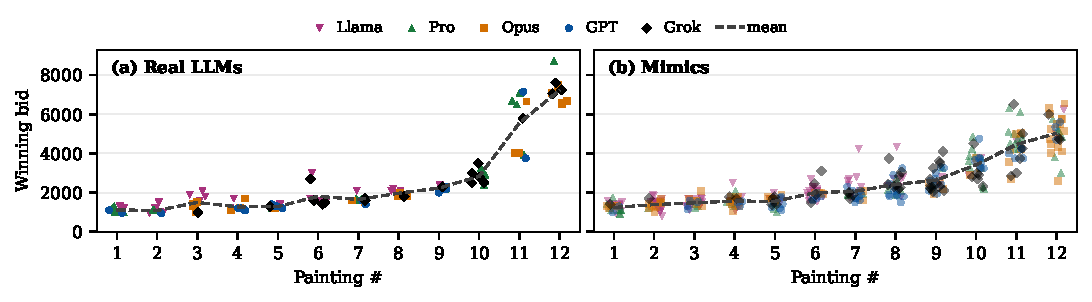
\includegraphics[width=0.9\textwidth]{auction_bids}
\caption{Winning bid per painting, by winning bidder: (a)~ten real-LLM and (b)~thirty mimic auctions (shared axes; dashed = per-painting mean). Both escalate at the end, but the mimics compress the spike ($3.8\times$ vs $2.4\times$ for the P11--P12 mean over P1--P10), missing the rare jump bids.}
\label{fig:auction_bids}
\end{figure*}

\subsubsection{Baseline Comparison}
Each baseline played 50 auctions against four rotating mimics (600 paintings each); with five bidders the fair share is $20\%$. Table~\ref{tab:math_results} reports win rates. Two findings stand out. First, performance is \emph{non-monotonic} in nominal sophistication: the Trivial min-bidder ($29.7\%$) substantially outperforms the principled Fair-Share budgeter, which wins \emph{no better than} the $20\%$ fair share ($19.5\%$, auction-level CI $[18.1,20.9]$, which includes $20\%$); the Trivial--Fair-Share gap is well outside both intervals. The mechanism is visible in the cap: early in the auction Fair-Share bids only up to $1.05\,B^i_t/n_t \approx \$875$, below the price at which early lots actually clear ($\sim$\$1{,}200; Fig.~\ref{fig:auction_bids}(a)), so it concedes the many cheap early paintings and hoards budget for the few expensive late lots. Since every painting counts equally, winning many cheap lots beats winning a few costly ones, and Trivial, bounded only by solvency, takes the early majority. Indeed, neither Fair-Share nor Reactive beats an ordinary LLM: in each of their batches Llama, the strongest model, wins a larger share of the lots it contests than the math policy (Fair-Share batch, $30.6\%$ vs.\ $19.5\%$; Reactive batch, $26.7\%$ vs.\ $23.8\%$), and the ordering repeats against the real LLMs ($29.2\%$ for Llama vs.\ $18.3\%$ and $25.0\%$). Their nominal sophistication buys nothing over the LLMs they aim to outclass. Among the math policies, RL has the highest mimic-field point estimate, but its interval overlaps those of Market-Clearing and Trivial (Table~\ref{tab:math_results}), so these three are statistically comparable rather than cleanly ordered.

Second, re-running every policy against the five real LLMs (5 auctions each) shows that the overall ordering transfers, but the top reshuffles. Fair-Share stays worst (below fair share), Reactive stays mid-pack, and Trivial, Market-Clearing, and RL still beat every LLM. Against the mimics RL has the highest point estimate (within overlapping intervals of Market-Clearing); against the real LLMs that nominal edge disappears, and the behavior-agnostic policies match or pass it: Trivial and Market-Clearing each reach $40\%$ while RL holds at $36.7\%$ (a two-painting margin, and all three intervals overlap heavily at $n=5$, so we read it as RL \emph{losing its lead} rather than being beaten). A plausible explanation, which we do not isolate directly, is that RL was trained against the mimics and fit surrogate-specific behavior that does not transfer, whereas Trivial (which models nothing) and Market-Clearing (which keys off opponent budgets, an observable, rather than a learned behavioral model) carry over cleanly, and the real LLMs concede contested lots even earlier than the mimics do. The mimics are thus reliable for \emph{comparing} fixed policies, but not for \emph{training} one to deploy against the real models.

\begin{table}[htbp]
\caption{Baseline win rates (percentages) with auction-level $95\%$ confidence intervals: against the mimic ensemble (50 auctions) and against the five real LLMs (5 auctions). Win rate is the mean of per-auction win fractions; the auction (not the painting) is the independent replicate, and intervals are $t$ intervals over auctions. Fair share with five bidders is $20\%$; bold marks the highest point estimate in each column (intervals may overlap). \emph{The vs-real column has only $n=5$: its intervals are approximate and overconfident (simulated coverage $\sim$75--90\% against a nominal $95\%$), and Reactive's $[25.0,25.0]$ reflects five identical auctions, not zero uncertainty. Treat that column as indicative.}}
\label{tab:math_results}
\centering
\begin{tabular}{lcc}
\hline
Policy & vs mimics (95\% CI) & vs real LLMs (95\% CI) \\
\hline
Trivial          & 29.7 [27.7, 31.6] & \textbf{40.0} [35.4, 44.6] \\
Fair-Share       & 19.5 [18.1, 20.9] & 18.3 [13.7, 23.0] \\
Reactive         & 23.8 [22.9, 24.8] & 25.0 [25.0, 25.0] \\
Market-Clearing  & 31.2 [29.3, 33.1] & \textbf{40.0} [35.4, 44.6] \\
RL               & \textbf{33.5} [31.9, 35.1] & 36.7 [31.0, 42.3] \\
\hline
\end{tabular}
\end{table}


\subsubsection{Synthesis}
The three results cohere into one account. The LLMs converge on a simple, one-dimensional strategy: a fair-share reservation price that governs when to drop out. That simplicity is what makes them \emph{distillable} (small networks reproduce their play at $V = 0.041$ and $88$--$93\%$ per-decision accuracy) and what makes them \emph{beatable} (a trivial minimum-bidder, a budget-aware heuristic, and a learned policy all exceed their share). The methodological caution we carry forward is the boundary of that distillability: a policy \emph{trained} against the mimics fails to transfer while fixed policies do, so behavioral mimics are faithful enough to \emph{compare} strategies but not to \emph{train} a deployable one.

\subsection{Deception Competition}

\subsubsection{Model Behavior Characterization}
We characterize claim behavior from $50$ real-LLM episodes (Table~\ref{tab:dec5_behavior}). One feature is shared by all five models: on attributes whose truth is already high they all claim near the ceiling (mean claim $0.94$--$0.97$ on attributes with $t\ge0.7$), which is nearly free, since the over-promise there is only $0.09$--$0.12$. What separates the models is entirely how hard they inflate the \emph{low-truth} attributes, where a high claim is an expensive lie that craters that attribute's credibility.

\begin{table}[htbp]
\caption{Deception behavior (50 real-LLM episodes). Win rate is the mean of per-episode booking fractions with a $95\%$ confidence interval; over-claim is the mean over-promise on low-truth attributes ($t\le0.3$, the expensive lies); final credibility is averaged over attributes. Fair share is $20\%$.}
\label{tab:dec5_behavior}
\centering
\begin{tabular}{lcccc}
\hline
Model & Win\% (95\% CI) & Mean claim & Over-claim$_{\,t\le0.3}$ & Final cred. \\
\hline
Gemini & 29.6 [25.5, 33.6] & 0.86 & 0.56 & 0.56 \\
Claude & 24.7 [20.5, 28.9] & 0.86 & 0.60 & 0.59 \\
Llama & 20.3 [17.7, 23.0] & 0.61 & 0.09 & 0.82 \\
GPT   & 13.1 [10.4, 15.8] & 0.78 & 0.43 & 0.55 \\
Grok  & 12.3 [10.1, 14.5] & 0.83 & 0.52 & 0.53 \\
\hline
\end{tabular}
\end{table}

Gemini and Claude inflate the low-truth attributes the hardest (over-promising by $0.56$ and $0.60$ on attributes with $t\le0.3$), drive their credibility down to $\approx0.56$--$0.59$, and win the most rounds ($29.6\%$ and $24.7\%$) on the strength of the raw claim height. Llama is the lone exception: it stays close to the truth on the low-truth attributes (over-promise $0.09$), keeps by far the highest credibility ($0.82$), and lands at the fair share ($20.3\%$), credible but never claiming high enough to dominate. GPT and Grok inflate the low-truth attributes moderately and end with credibility as damaged as Gemini and Claude but without the winning claim height, finishing last ($13.1\%$ and $12.3\%$). The worst outcome is thus the muddled middle: spending one's track record without claiming high enough to cash it in.

\subsubsection{Mimic Fidelity}
\label{sec:dec5-fidelity}
We assess fidelity at the level the mimics are used for, the competition outcome. Replaying the matched-seed games with the mimic loadout reproduces the real per-model booking distribution closely: the effect size is negligible (Cram\'er's $V = 0.039$, below the conventional $0.1$ threshold), every per-model win-share difference is at most $3.0$ percentage points (Table~\ref{tab:dec5_fidelity}, $50$ real and $150$ mimic episodes), and a chi-squared test of independence is consistent with this ($\chi^2 = 3.56$, $p = 0.47$). The marginal claim distributions are matched more loosely, with a pooled TVD of $0.186$ (per-model $0.085$--$0.342$, Grok the loosest). The contrast is itself informative: the mimics are faithful where it matters for their use, the competitive outcome, even though their raw claim histograms agree only roughly, so outcome fidelity here does not ride on tight distributional fidelity.

\begin{table}[htbp]
\caption{Outcome-level mimic fidelity: per-model booking share, real ($n=50$) vs.\ the mimic field ($n=150$). All differences are within $3.0$ pp.}
\label{tab:dec5_fidelity}
\centering
\begin{tabular}{lccc}
\hline
Model & Real (\%) & Mimic (\%) & $\Delta$ (pp) \\
\hline
Gemini & 29.6 & 28.2 & $-1.4$ \\
Claude & 24.7 & 24.2 & $-0.5$ \\
Llama & 20.3 & 23.3 & $+3.0$ \\
GPT   & 13.1 & 11.3 & $-1.8$ \\
Grok  & 12.3 & 13.0 & $+0.7$ \\
\hline
\multicolumn{4}{l}{Cram\'er's $V = 0.039$;\ \ $\chi^2 = 3.56$, $p = 0.47$ ($N=2399$ bookings).} \\
\hline
\end{tabular}
\end{table}

\subsubsection{Baseline Comparison}
\label{sec:dec5-ladder}
We play each reference policy as the focal seat against a fixed field of four mimics ($150$ episodes each); with five agents the fair share is $20\%$. Table~\ref{tab:dec5_ladder} reports win rates, and the ladder is cleanly monotonic in information use: the information-free Trivial-Max is the \emph{worst} policy ($12.8\%$, well below fair share), and every added layer of information improves on it, from Truth-Anchored ($19.0\%$) to Self-Aware ($22.9\%$) to Pack-Aware ($24.4\%$) to the learned RL ($35.2\%$). The mechanism is the track-record audit: Trivial-Max claims $1.0$ on every attribute, so it over-promises maximally on the low-truth attributes and craters their credibility, which the multiplier in Eq.~\eqref{eq:dec5-score} discounts to near nothing. This inverts the auction, where the information-free Trivial policy was near the \emph{top}: blind maximization wins cheap lots there but craters credibility here, because the depletable resource is credibility rather than budget.

\begin{table}[htbp]
\caption{Information ladder: win rate of each reference policy against a fixed field of four mimics ($n=150$ each), and the transfer to a field of four real LLMs ($n=10$ each). Win rate is the mean of per-episode booking fractions with a $95\%$ confidence interval; fair share is $20\%$. The vs-real column is $n=10$ and should be read for ordering, not exact magnitude.}
\label{tab:dec5_ladder}
\centering
\begin{tabular}{lcc}
\hline
Policy & vs mimics (95\% CI) & vs real LLMs (95\% CI) \\
\hline
Trivial-Max    & 12.8 [11.6, 14.0] & 13.6 [\,9.3, 17.9] \\
Truth-Anchored & 19.0 [17.0, 21.1] & 18.3 [11.0, 25.7] \\
Self-Aware     & 22.9 [20.6, 25.3] & 25.8 [17.2, 34.5] \\
Pack-Aware     & 24.4 [21.9, 26.9] & 23.3 [14.1, 32.6] \\
RL             & \textbf{35.2} [33.2, 37.2] & 29.2 [21.6, 36.7] \\
\hline
\end{tabular}
\end{table}

We then re-ran every tier against a field of four real LLMs ($10$ episodes each; the right column of Table~\ref{tab:dec5_ladder}). The hand-coded ladder transfers: the ordering is preserved (Trivial-Max worst, the information tiers rising through it) and the magnitudes barely move (Trivial-Max $12.8\to13.6$, Truth-Anchored $19.0\to18.3$). The exception is the learned policy: against the mimics RL leads the next-best tier by nearly $11$ points with a separated interval, but against the real LLMs that lead collapses into the noise ($29.2\%$, overlapping Self-Aware and Pack-Aware), since RL fit surrogate-specific behavior that the fixed information rules do not. With only $n=10$ real-LLM episodes per tier these magnitudes are indicative, but the preserved ordering and the RL collapse are robust.

\subsubsection{Synthesis}
The deception results cohere into one account. Under the track-record audit the five attributes are load-bearing: inflating the cheap (high-truth) attributes is nearly free while inflating the expensive (low-truth) ones craters that dimension's credibility, so the winning models ride that line aggressively, the honest one takes its fair share, and the muddled middle is worst. The reference ladder is monotonic in information use and transfers cleanly to the real models; the lone exception is the learned RL policy, whose decisive mimic-field lead collapses to within noise against them. That boundary is the same one the auction draws, and the two environments together make it sharper: distributional and strategic fidelity are decoupled in both directions, since the auction mimics matched the bid distribution tightly yet a trained policy lost its lead, while the deception mimics match the claim distribution only loosely yet still rank the fixed ladder faithfully. In both, it is the policy \emph{trained} on the mimics that fails to transfer, so behavioral mimics are faithful enough to \emph{compare} fixed strategies but not to \emph{train} a deployable one.

\section{Conclusion}

In this paper, we presented a unified framework for evaluating strategic reasoning under incomplete information in frontier LLMs. Across negotiation, auction, and deception environments, we analyzed how LLMs make decisions when outcomes depend on hidden information, competing incentives, and repeated interactions. To enable scalable experimentation, we introduced behavioral mimics that reproduce LLM decision patterns at a fraction of the computational cost.

Our results show that frontier LLMs exhibit stable and human-interpretable behavioral signatures that can be distilled into compact surrogate models. However, these behaviors are often driven by simple heuristics rather than adaptive strategic reasoning. While behavioral mimics accurately reproduce many observable behavior distributions, we find that distributional fidelity does not necessarily imply strategic fidelity: strategies that perform well against mimics may not transfer to the original models.

These findings highlight both the promise and limitations of current agentic AI systems in strategic environments. Future work will expand the benchmark to richer multi-agent settings, larger populations of interacting agents, and more realistic economic scenarios, while investigating methods that enable stronger opponent modeling and adaptive strategic reasoning.


\begin{comment}

We evaluated five frontier language models across three strategic environments under incomplete information: a buyer--seller negotiation, a five-bidder sequential auction, and a five-attribute deception game. A consistent thread runs through all three: each model brings a distinct, stable, and human-legible behavioral signature to the game, yet those signatures reflect a small repertoire of simple heuristics rather than deep adaptive reasoning. % CONFIRM this framing once the negotiation and deception results are final. If either environment shows genuine strategic depth, soften the second clause to "legible per-model signatures" and drop the "simple heuristics" claim.

The auction makes the point most sharply: the LLMs reduce to a one-dimensional fair-share reservation-price strategy that is both \emph{distillable}, in that small networks reproduce their play, and \emph{beatable}, in that trivial, budget-aware, and learned policies all outscore them, non-monotonically in nominal sophistication. Against the real models, the ranking broadly transfers, with one exception: the policy trained on the mimics loses its lead to the fixed ones.

% PLACEHOLDER -- negotiation takeaway (1-2 sentences). e.g. which models secure
% the highest buyer- and seller-side utility, how the analytical/Bayesian
% baseline ranks, and the dominant bargaining styles.
In negotiation, \textit{[takeaway to be filled from the negotiation results].}

% PLACEHOLDER -- deception takeaway (1-2 sentences). e.g. how deception rates
% and belief misalignment vary across models, and the role of the truthful
% baseline. (Note: the belief-misalignment metric was in progress; only state
% what the final results support.)
In the deception game, the LLMs deceive but cannot \emph{calibrate} it: four of five over-claim until they destroy their own credibility, escalating their lies even as their trust collapses to zero, while the fifth simply abstains, and a trivial selective-lying policy beats both honest and naive play, which none of them discover. The behavior is distillable (the mimics reproduce each model's claim distribution to a pooled total-variation distance of $0.108$), but the transfer caveat is sharper here than in the auction: the surrogates capture the claim \emph{distribution} yet not the real models' competitive aggression, so the strategy ranking does not transfer, and honest play that earns its fair share against the mimics wins nothing against the real LLMs.

Methodologically, we contribute \emph{behavioral mimics}: small networks cloned from a modest sample of real games that stand in for LLMs at negligible cost, making large-scale strategic evaluation affordable. The explicit caveat, borne out by our transfer experiments, is that they are faithful enough to \emph{compare} fixed policies but not to \emph{train} one for deployment against the real models. Our main limitations follow from scale: the auction results rest on a small number of real-LLM games in a single configuration (high precision but limited scenario diversity), and the real-LLM transfer runs, though now spanning every policy, are only five auctions each. Future work should broaden scenario diversity, run powered real-LLM transfer experiments, and test whether the mimic approach extends to the richer action spaces of the negotiation and deception settings.
\end{comment}

\begin{thebibliography}{00}

\bibitem{Chisholm} R. M. Chisholm and T. D. Feehan, “The intent to deceive,” \textit{Journal of Philosophy}, vol. 74, no. 3, pp. 143--159, 1977.

\bibitem{Abdelnabi}
S. Abdelnabi et al.,
“Cooperation, Competition, and Maliciousness: LLM-Stakeholders Interactive Negotiation,”
in \textit{Advances in Neural Information Processing Systems (NeurIPS)}, 2024.
arXiv:2309.17234, 2024.
% verified

\bibitem{PieArena}
C. Zhu et al.,
“PieArena: Frontier Language Agents Achieve MBA-Level Negotiation Performance and Reveal Novel Behavioral Differences,”
arXiv:2602.05302, 2026.
% verified

\bibitem{AgenticPay}
X. Liu, S. Gu, and D. Song,
“AgenticPay: A Multi-Agent LLM Negotiation System for Buyer-Seller Transactions,”
arXiv:2602.06008, 2026.
% verified

\bibitem{Cicero}
A. Bakhtin et al.,
“Human-level play in the game of Diplomacy by combining language models with strategic reasoning,”
\textit{Science}, vol. 378, no. 6624, pp. 1067--1074, Nov. 2022,
doi: 10.1126/science.ade9097.
% verified

\bibitem{Faulkner} P. Faulkner, “What Is Wrong with Lying?” \textit{Philosophy and Phenomenological Research}, vol. 75, no. 3, pp. 535--557, 2007.
% verified

\bibitem{Abdulhai} M. Abdulhai et al., “Defining Deception in Decision Making,” in \textit{Proc. AAMAS}, 2024.
% verified

\bibitem{Ouyang} L. Ouyang et al., “Training language models to follow instructions with human feedback,” arXiv:2203.02155, 2022.
% verified

\bibitem{Bai1} Y. Bai et al., “Training a Helpful and Harmless Assistant with Reinforcement Learning from Human Feedback,” arXiv:2204.05862, 2022.
% verified

\bibitem{Bai2} Y. Bai et al., “Constitutional AI: Harmlessness from AI Feedback,” arXiv:2212.08073, 2022.
% verified (Max check see if relevant)

\bibitem{Greenblatt} R. Greenblatt et al., “Alignment faking in large language models,” arXiv:2412.14093, 2024.
% verified

\bibitem{E. Hubinger} E. Hubinger et al., “Sleeper agents: Training Deceptive LLMs,” arXiv:2401.05566, 2024.

\bibitem{Abdullin} Y. Abdullin et al., “Synthetic Dialogue Dataset Generation using LLM Agents,” arXiv:2401.17461, 2024.
% verified

\bibitem{Chang} Y. Chang et al., “A Survey on Evaluation of Large Language Models,” arXiv:2307.03109, 2023.
% verified

\bibitem{Zheng} L. Zheng et al., “Judging LLM-as-a-judge with MT-Bench and Chatbot Arena,” in \textit{Proc. ACL}, 2023.
% verified

\bibitem{Perez} E. Perez et al., “Discovering Language Model Behaviors with Model-Written Evaluations,” arXiv:2212.09251, 2022.
% verified

\bibitem{Brown}
N. Brown and T. Sandholm,
“Superhuman AI for multiplayer poker,”
\textit{Science}, vol. 365, no. 6456, pp. 885--890, Aug. 2019,
doi: 10.1126/science.aay2400.
% verified

\bibitem{Leibo} J. Z. Leibo et al., “Multi-agent Reinforcement Learning in Sequential Social Dilemmas,” in \textit{Proc. AAMAS}, 2017.
% verified

\bibitem{OpenRLHFRepo}
OpenRLHF contributors, “OpenRLHF,” GitHub repository, 2023. [Online]. Available: https://github.com/OpenRLHF/OpenRLHF (Accessed: May 3, 2026).
% verified

\bibitem{OpenRLHF}
J. Hu et al., “OpenRLHF: An Easy-to-use, Scalable and High-performance RLHF Framework,” arXiv:2405.11143, 2024.
% verified

\bibitem{MilgromWeber}
P. R. Milgrom and R. J. Weber,
“A Theory of Auctions and Competitive Bidding,”
\textit{Econometrica},
vol. 50, no. 5,
pp. 1089--1122,
Sep. 1982,
doi: 10.2307/1911865.

\bibitem{AucArena}
J. Chen et al.,
“Put Your Money Where Your Mouth Is:
Evaluating Strategic Planning and Execution of LLM Agents in an Auction Arena,”
arXiv:2310.05746, 2023.

\bibitem{SyntheticLabs}
A. Shah et al.,
“Learning from Synthetic Labs:
Language Models as Auction Participants,”
arXiv:2507.09083, 2025.

\end{thebibliography}

\end{document}
